%
%
%
%
\chapter{Preconditioned Agglomeration Multigrid for Hybrid Grids}
\label{multigrid.chap}
\headc{Preconditioned agglomeration multigrid}
\setcounter{footnote}{0}
%
%
%
 A preconditioned directional-implicit agglomeration multigrid method
 has been developed for the solution of the linear and non-linear
 Navier-Stokes equations on highly anisotropic unstructured hybrid grids
 in 2D and 3D. The coarse grid levels are constructed
 automatically from the fine grid by agglomerating fine grid control
 volumes together. Since the coarse grid control volumes may have arbitrary
 polygonal shapes, the type of elements constituting the fine grid is
 irrelevant. In this way the discrete equations on coarse grid levels
 are assembled automatically without the explicit creation of a coarse grid.
 The multigrid smoother consists of a preconditioned
 point- or line-Jacobi Runge-Kutta relaxation algorithm, which guarantees
 efficient damping of high frequency error modes on highly stretched grids.
%
%
%
%
\section{Introduction}
\headd{Agglomeration Multigrid}{Introduction}
%
 The basic idea of a multigrid strategy
 is to obtain a faster rate of development of the solution on a fine grid
 by approximating the fine-grid problem on successively coarser grids.
 With suitable coarse-grid approximations of the fine-grid problem, the
 low-frequency error components on the fine grid appear as high-frequency
 error components on the coarser grids. The low-frequency components on the
 fine grid, where the discrete solution is desired, are precisely the error
 components that dramatically slow down the convergence of single-grid schemes.
 There are two additional advantages derived from displacing part of the
 effort in solving a set of discrete equations to coarse grids.
 First, a larger mesh spacing permits larger time steps thus allowing a faster
 propagation of the informations in the domain of interest.
 This point is of particular importance for convection dominated problems
 such as the ones described by the Euler and Navier-Stokes equations.
 Such equations exhibit both elliptic and hyperbolic properties in their
 discrete formulations meaning that the coarse meshes in the multigrid cycle
 serve the dual role of enhancing both damping and propagation of error
 modes.
 Another advantage of the coarse grids is that they require less computational
 effort because of the reduced degrees of freedom involved compared with
 the fine grid. For example, in 2D the computational effort needed
 is decreased roughly by a factor of four on successively coarser meshes.

 Multigrid methods have proven to be very effective techniques for accelerating
 convergence to steady state of both elliptic and hyperbolic problems.
 For simple elliptic problems, such as a Poisson equation, convergence rates of
 0.1 are achievable, meaning that for each multigrid cycle, the numerical error
 can be reduced by one order of magnitude (Mavriplis \citeyearNP{Mavriplis:6}).
 For hyperbolic problems, such as the Euler equations, the best rate
 that theoretically can be achieved for a second order discretisation is
 0.75, according to the analysis discussed by Mulder \citeyear{Mulder:2}.

 On the other hand, the development of efficient numerical methods for the
 solution of the high-Reynolds number viscous flow remains one of the ongoing
 challenge in the field of computational fluid dynamics. Multigrid Navier-Stokes
 solvers generally result in convergence rates which are an order of magnitude
 or more slower than those obtained for inviscid flows
 (Mavriplis \citeyearNP{Mavriplis:7}, Pierce \& Giles \citeyearNP{Giles:10}).
 The main reason for this breakdown in efficiency
 of the multigrid algorithm stems from the need to use a computational mesh
 that is highly resolved in the direction normal to the wall in order to
 accurately represent the steep gradients in the boundary layer.
 Indeed, the higher the Reynolds number, the more grid stretching is required,
 and the worse the convergence rate becomes. The design of an appropriate
 numerical approach must therefore be based on a careful assessment of the
 interaction between the discrete method, the computational mesh and the physics
 of the viscous flow.

 Over the last few years, different methods have been proposed to overcame
 the increased stiffness of the discrete system of equations due to high
 aspect ratio cells. Mulder \citeyear{Mulder:1} proposed a semi-coarsening
 multigrid strategy in which the mesh is coarsened only in the direction
 normal to the grid stretching, rather then in all coordinate simultaneously.
 One major drawback of semi-coarsening techniques is that they results
 in coarse grids of higher complexity. While full coarsening approach
 reduces grid complexity between successively coarser levels by a factor of 4 in
 2D, and 8 in 3D, semi-coarsening techniques only achieve a grid complexity
 reduction of 2, in both 2D and 3D. This increase the costs of a multigrid
 cycle especially in 3D.
 More recently Pierce \& Giles \citeyear{Giles:10} and
 Pierce et al. \citeyear{Giles:11} have proposed preconditioning
 methods, coupled with explicit multistage scheme, as a less expensive approach
 to overcoming multigrid breakdown in the presence of boundary layer
 anisotropy.

 Following the analysis by Pierce et al. \citeyear{Giles:11},
 two different form of preconditioner were implemented in the
 numerical method presented in this research project.
 These preconditioners are either the point- or line-Jacobian matrix obtained
 through a linearisation of the first order discretisation of the
 Navier-Stokes equations. In 3D the point-Jacobian preconditioner is a
 block-matrix $5\times5$ which can be directly inverted at a reasonable costs.
 Mavriplis \citeyear{Mavriplis:6,Mavriplis:7} reviews these multigrid
 strategies for viscous
 flow solvers on anisotropic hybrids grids in the context of agglomeration
 multigrid.
%
%
%
%
\section{Algorithm Description}
\headd{Agglomeration Multigrid}{Algorithm description}
%
 The main difficulty with multigrid techniques on hybrid unstructured grids
 is the generation of coarse grids. On structured grids, a sequence of grids
 can be constructed trivially by omitting alternate grid points in each
 direction. In the case of unstructured grid four main approaches can be
 adopted. The first strategy is to produce a sequence of fine grids
 from a coarse grid by refinement. The advantage is that the inter-grid
 operators become simple because of the nesting of the grid. The major drawback
 of such method is the predetermination of the coarsest level in the multigrid.
 This may be too fine if the geometry is to be captured on the coarse grid.
 Another method, labelled non-nested multigrid, uses a sequence of
 grids which are generated independently by a grid generator.
 Piecewise-linear interpolation operators for the transference of flow
 variables, residuals and correction are derived during a pre-processing stage
 by using efficient search procedures. Non-nested multigrid method
 has been shown to be quite successful on unstructured grid computations
 (Peraire et al. \citeyearNP{Peiro:3}). However, the generation of the sequence
 of grid is not automatic and requires a robust mesh generator. In addition, the
 development of efficient Piecewise-linear interpolation operators on hybrid
 grid is not a straightforward task.
 A third approach is the edge collapse multigrid which uses
 an automatic point removal algorithm to
 generate a sequence of coarse grids from an initial fine grid. This is
 completely automatic and has been successfully adopted for hybrid unstructured
 meshes (Moinier et al. \citeyearNP{Giles:9}).

 A completely different approach is the generation of coarse grids through
 agglomeration as developed by Mavriplis \& Venkatakrishnan
 \citeyear{Mavriplis:3,Mavriplis:8}. The central idea of agglomeration multigrid
 is to form coarse grid levels by fusing fine grid control volumes together
 as shown in Fig. \ref{agglo1.fig}. Since the coarse grid levels may have
 arbitrary polygonal shapes (polyhedral in 3D), the type of elements constituting
 the fine grid is irrelevant.

%
\begin{figure}[ht]
   \centerline{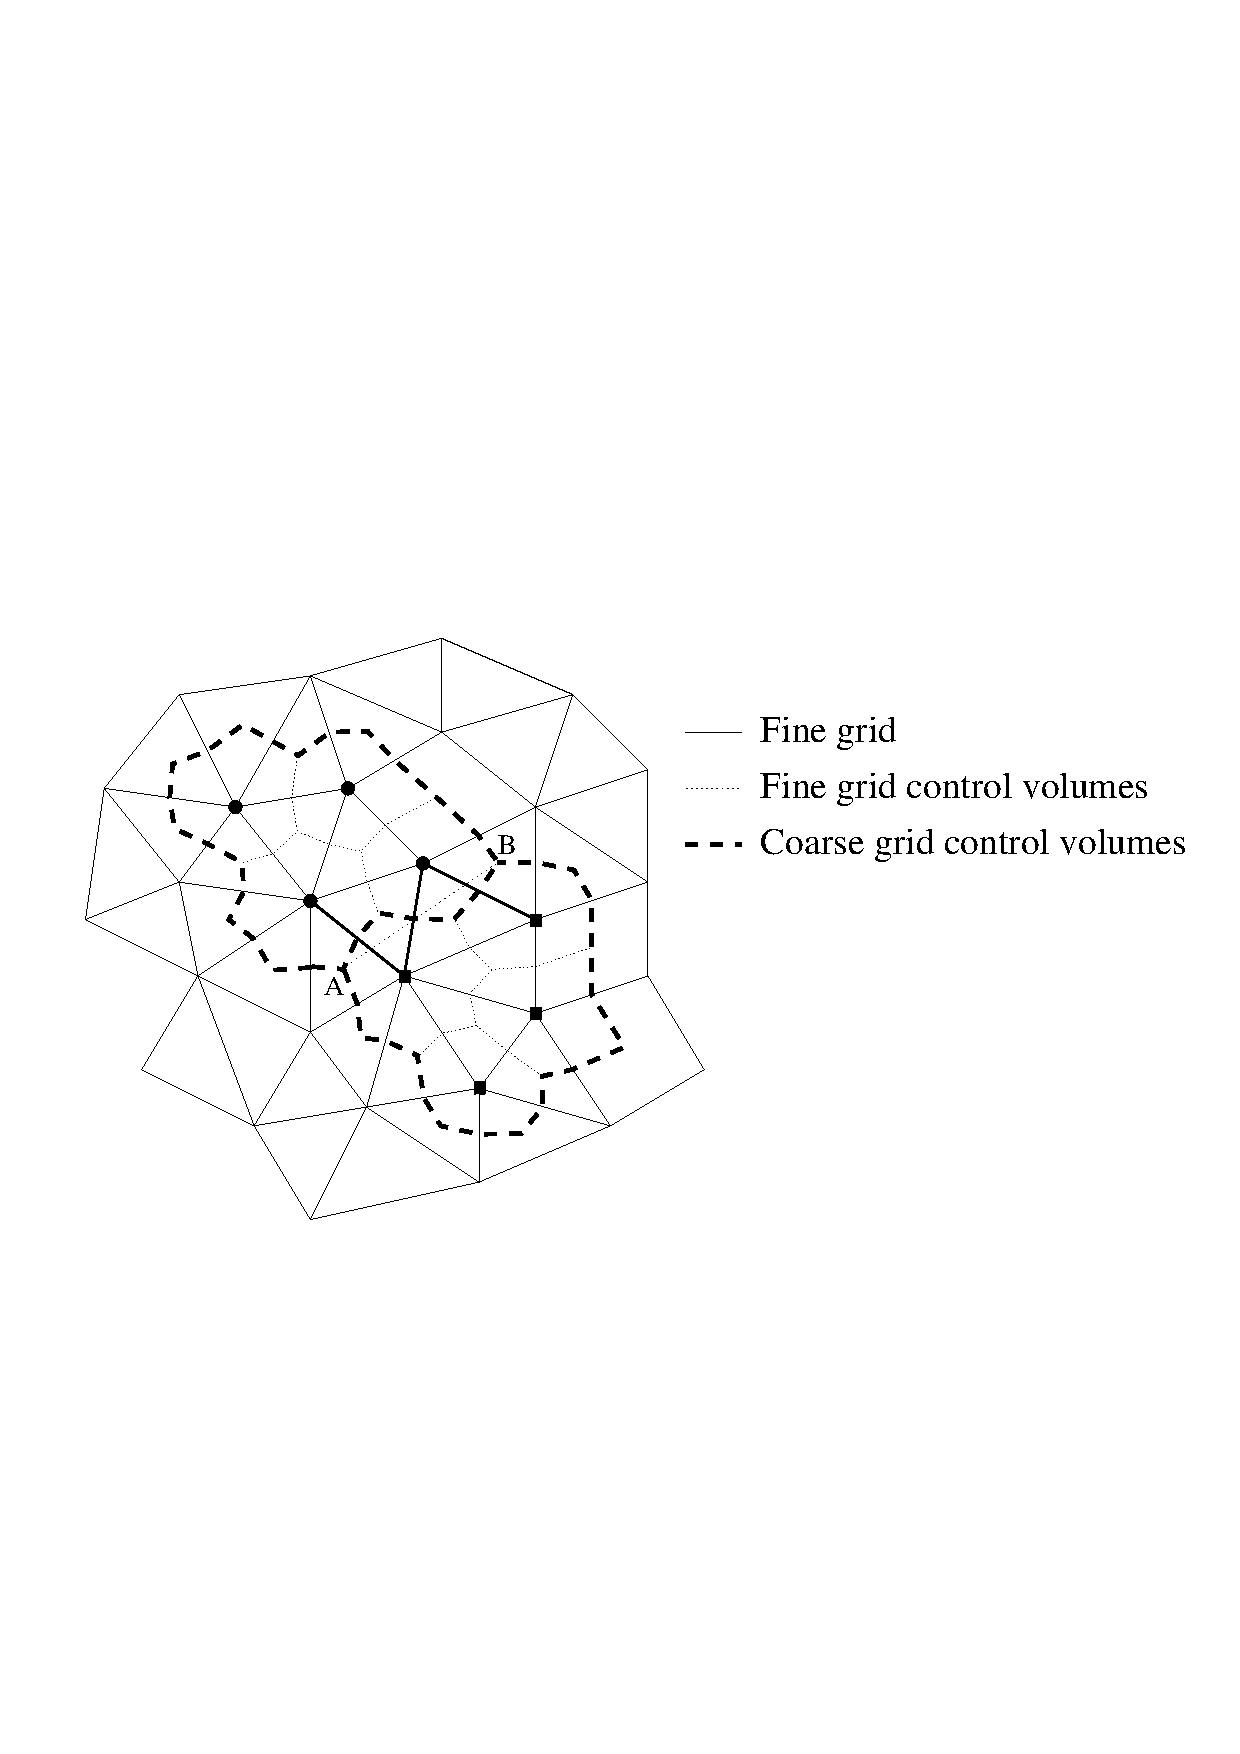
\includegraphics[width=100mm,clip=t]{APPEND/FIGURE/aggloc.pdf}}
   \caption{Example of two agglomerated coarse grid volumes}
   \label{agglo1.fig}
\end{figure}
%
 An edge-based solver performs all the operations utilizing the volumes and edge
 coefficients only, thus it can handle an arbitrary polyhedral coarse grid
 in a straightforward way. The fluxes in the coarse grid levels are evaluated
 using a the first-order Roe'upwind solver for polyhedral grids developed by
 Barth \& Jespersen \citeyear{Barth:1}.

 The agglomeration procedure can be interpreted as a Galerkin coarse grid
 approximation (Wesseling \citeyearNP{Wesseling:1}). Agglomeration can thus
 viewed as identifying all of the fine grid cells with the coarse cell to
 which they belong, and then summing the equations corresponding to these cells.
 Interpreted in this manner, agglomeration multigrid is similar to
 algebraic multigrid procedure. In a purely algebraic multigrid, which is
 strictly valid for linear system, no underlying
 grid is defined, and only the matrix ${\bf A}$ of a linear system
 ${\bf A}s = b$ is known. The coarse grid operator is then obtained by a direct
 summation of the non-zero entries in the fine level matrix. Agglomeration
 multigrid represents an extension of these ideas to non-linear systems.
 In this approach, only the solution independent terms are summed in going
 from fine to coarse levels. For example in Fig. \ref{agglo1.fig}, edge
 AB represents the summation of the edge vector in the fine grid
 which are common between the two coarse agglomerated cells.
 The solution dependent terms are obtained from coarse level variables
 interpolated up from the fine level solution, following a Full
 Approximation Storage scheme (FAS).
%
%
%
\subsection{FAS scheme}
%
 In this section a description of the full approximation storage (FAS) multigrid
 scheme is given.
 Suppose that successively coarser agglomerated grids are introduced, with the
 grids numbered from 1 to $K$, where grid 1 is the original mesh.
 For $k > 1$, the evolution on grid $k$ is driven by a weighted average of
 the residuals calculated on grid $k-1$, so that each mesh simulates the
 evolution that would have occurred on the next finer mesh
 (Jameson \citeyearNP{Jame:4}, Wesseling \citeyearNP{Wesseling:1}).
 When the coarsest grid has been reached, changes in the solution calculated
 on each mesh are consecutively interpolated back to the next finer grid.

 The fine grid system of equations is written for both steady-state
 and unsteady nonlinear flow as well as linearised unsteady flow, as:

%
\beq
  \left[{\bf P}\right]\se{-1}L\sm{\tau} \delta{\bf U} = {\bf R}\left({\bf U}\right)
  \label{fine_grid.eq}
\eeq
%
 with $L\sm{\tau}$ indicating the pseudo time-marching Runge-Kutta operator.
 The discrete system of equations for a general grid $k$ can be written as

%
\beq
  \left[{\bf P}\right]\se{-1}L\sm{\tau} \delta{\bf U}\se{k} &=& {\bf R}\se{k} - {\bf F}\se{k}
  \label{coarse_grid1.eq}
\eeq
%
 where ${\bf F}\se{k}$ represents the multigrid forcing function which is needed
 in order to simulates the evolution process in the finer grid.
 This forcing function is zero for the finer grid ($k = 1$) while for $k > 1$
 it assumes the following form:

%
\beq
  {\bf F}\se{k} &=& {\bf R}\left({\bf U}\se{k}\sm{old}\right) -
                          \Theta\sm{\tt Res}\se{R^{k-1\rightarrow k}}
                          \left({\bf R}\left({\bf U}\sm{old}\se{k-1}\right) -
                                {\bf F}\se{k-1}\right)\\
  {\bf U}\se{k}\sm{old} &=& \Theta\sm{\tt Unk}\se{R^{k-1\rightarrow k}}
                            {\bf U}\se{k-1}\sm{old}
  \label{forcing_term.eq}
\eeq
%
 The symbol $\Theta$ represent inter-grid transfer operators which will be
 defined shortly. The coarse grid equations are solver for ${\bf U}\se{k}$
 with starting solution ${\bf U}\se{k}\sm{old}$. The correction are then
 interpolated back to the fine grid as

%
\beq
  {\bf U}\se{k-1}\sm{new} =
  {\bf U}\se{k-1}\sm{old} + \Theta\se{P^{k\rightarrow k-1}}
 \left({\bf U}\se{k}\sm{new} - {\bf U}\se{k}\sm{old}\right)
\eeq
%
 One of the principal advantages of this FAS algorithm is that it
 enables an efficient solution
 strategy which requires little more memory than that of the single
 grid solver (Wesseling \citeyearNP{Wesseling:1}).

 A recursive algorithm, which allows the use of an arbitrary number
 of meshes in either a V or W type cycles, has been implemented following
 the approach by Peraire et al. \citeyear{Peiro:3}.
%
%
%
\subsection{Transfer Operators}
%
 Three inter-grid transfer operators need to be defined in order
 to have a complete description of the algorithm.
%
\paragraph{Restriction:} transfers the solution and residual vector
 from fine to coarse grids. Here a simple injection has been employed.

%
\beq
  \Theta\sm{\tt Unk}\se{R^{k-1\rightarrow k}}
  {\bf U}\se{k-1} &=&
  \frac{1}{{\cal V}\se{k}}
  \sum_{c=1}^{n_c} \left({\cal V}{\bf U}\right)\sm{I_c}\se{k-1}
  \label{restriction1.eq}\\
  \Theta\sm{\tt Res}\se{R^{k-1\rightarrow k}}
  {\bf R}\se{k-1} &=&
  \sum_{c=1}^{n_c} {\bf R}\sm{I_c}\se{k-1}
  \label{restriction2.eq}
\eeq
%
 where $n\sm{c}$ represents the number of control volumes in the fine grid
 $k-1$ contained in the agglomerated coarse grid control volume.
 In Fig. \ref{agglo1.fig} shows two agglomerated coarse control volumes
 which contains four fine control volumes each.
%
%
\paragraph{Prolongation:} transfers the change of the solution from
 coarse to fine grid. Since a set of fine control volumes are included
 in one coarse agglomerated cell only, a simple copy of the coarse
 grid correction has been used.

%
\beq
  \Theta\se{P^{k\rightarrow k-1}}
  \left(\Delta{\bf U}\se{k}\right) &=& \Delta{\bf U}\se{k}
  \label{prolongation.eq}
\eeq
%
 Multigrid theory (Wesseling \citeyearNP{Wesseling:1}) suggests that

%
\beq
  m\sm{R} + m\sm{P} > m\sm{E}
  \label{multigrid_theory.eq}
\eeq
%
 where $m\sm{R}$ and $m\sm{P}$ are the order of polynomial that
 the restriction and the prolongation can transfer exactly, and $m\sm{E}$
 is the order of the differential equation, which is 2 for the
 Navier-Stokes equations.
 Both transfer operators described in (\ref{restriction1.eq}) and
 (\ref{prolongation.eq}) can transfer correctly only first order
 polynomial, thus violating (\ref{multigrid_theory.eq}) in the case of
 Navier-Stokes equations.
 Unfortunately, devising higher order transfer operators in the case
 of agglomerated grids is non-trivial because of the absence of an
 underlying grid. However, the use of an efficient smoother can
 alleviate such a drawback by being effective in removing
 high-frequency errors resulting from the corrections from the fine-grid
 approximation.
%
%
%
%
%
\section{Smoother}
\headd{Agglomeration Multigrid}{Smoother}
%
 Having established the multigrid strategy and the transfer operators
 to be used, it remains to define the smoother $L\sm{\tau}$ in (\ref{fine_grid.eq}).
 Efficient multigrid performance  relays heavily on the ability of
 the smoother to damp on the current mesh all the modes
 that cannot be resolved without aliasing on the next coarser mesh
 in the cycle (Pierce \& Giles \citeyearNP{Giles:10}). Moreover for
 hyperbolic problems, the smoother must enhance the propagation of
 error modes outside the computational domain.
 Broadly speaking, relaxation methods are traditionally classified into
 explicit and implicit scheme. Explicit scheme offers a low operation count,
 low storage requirements but they suffer from limited stability imposed by
 the CFL conditions. Implicit schemes theoretically offer unconditional
 stability and presumably insensitiveness to the degree of anisotropy in
 the problem to be solved.
 In practice direct implicit method are infeasible for large 3D problems due
 to high operation counts and memory requirements so that the inversion
 of the Jacobian matrix must be performed using iterative or approximate
 factorization techniques.
 Such techniques are only moderately implicit and are not efficient when
 very large time-steps are employed so that it is not possible to benefits
 the unconditional stability. Moreover such schemes, often design for
 isotropic problems, degrade with increasing anisotropy.
 Here an efficient solution strategy for highly anisotropic problems
 based on preconditioned point-Jacobi or line-Jacobi multistage Runge-Kutta scheme
 has been employed.
%
%
%
\subsection{Time-stepping}
%
 From (\ref{time_steadystate.eq}), (\ref{Dual_time_stepping_3.eq}) and
 (\ref{time_linear.eq}), the the semi-discrete finite
 volume discretisation of the Navier-Stokes system of equations appears as
%
\beq
  \left[{\bf P}\right]\se{-1} L\sm{\tau} {\bf U}\sm{I} =
  {\bf R}\sm{I}\left({\bf U}\right)
 \label{Time_stepping_1.eq}
\eeq
%
 where $\left[{\bf P}\right]\se{-1}$ is the preconditioner.
 A Q-stage scheme for the grid level $k$ can be written as:

%
\beq
  {\bf U}\se{k}\sm{0} &=& {\bf U}\se{k}\sm{old} \nonumber \\
   &\vdots& \nonumber\\
  {\bf U}\se{k}\sm{q+1} &=& {\bf U}\se{k}\sm{0} +
  \alpha\sm{q} \left[{\bf P}\right] \left({\bf R}\se{k}\sm{q} - {\bf F}\se{k}\right)
  \label{runge_kutta.eq}\\
   &\vdots& \nonumber\\
  {\bf U}\se{k}\sm{new} &=& {\bf U}\se{k}\sm{Q} \nonumber
\eeq
%
 where $\alpha\sm{q}$ are the Runge-Kutta parameters.
 Throughout this work the five-stage Runge-Kutta scheme of Jameson
 \citeyear{Jame:2} with alternate evaluation of the physical and artificial
 dissipation has been used.
 If one indicates with ${\bf Q}\se{k}\sm{q}$ the convective part and with
 ${\bf D}\se{k}\sm{q}$ the dissipation part of the residual ${\bf R}\se{k}\sm{q}$
 in (\ref{runge_kutta.eq}) then from Jameson \citeyear{Jame:2}

%
\beq
  {\bf Q}\se{k}\sm{q} &=& {\bf Q}\left({\bf U}\se{k}\sm{q}\right) \nonumber\\
  {\bf D}\se{k}\sm{q} &=& \beta\sm{q}{\bf D}\left({\bf U}\se{k}\sm{q}\right)
                       + \left(1-\beta\sm{q}\right){\bf D}\se{k}\sm{q-1}
  \label{rk_residual.eq}\\
  {\bf R}\se{k}\sm{q} &=& {\bf Q}\se{k}\sm{q} + {\bf D}\se{k}\sm{q} \nonumber
\eeq
%
 If one reduces the linear model corresponding to (\ref{runge_kutta.eq}) to
 an ordinary differential equation and indicates with
 $\widehat{\bf U}\sm{new} = \psi\left(Z\right) \widehat{\bf U}\sm{old}$ the
 Fourier amplitude evolution,
 where $\left|\psi\left(Z\right)\right|$ is the amplification factor of the
 integration, the resulting Fourier symbol has an imaginary part which is
 proportional to the wave speed and a negative real part proportional to
 the diffusion.
 The coefficients $\alpha\sm{q}$ in (\ref{runge_kutta.eq}) are chosen to
 maximize the stability interval along the imaginary axis and $\beta\sm{q}$
 are chosen to increase the stability interval along the negative real axis.
 The five-stage scheme which has been found to be particularly effective
 (Jameson \citeyearNP{Jame:2}) has coefficients
%
\beq
\begin{array}{rclcrcl}
 \alpha\sm{1} & = & 1/4 & \hspace{5mm} & \beta\sm{1} & = & 1\\
 \alpha\sm{2} & = & 1/6 & \hspace{5mm} & \beta\sm{2} & = & 0\\
 \alpha\sm{2} & = & 3/8 & \hspace{5mm} & \beta\sm{3} & = & 0.56\\
 \alpha\sm{2} & = & 1/2 & \hspace{5mm} & \beta\sm{4} & = & 0\\
 \alpha\sm{2} & = & 1   & \hspace{5mm} & \beta\sm{5} & = & 0.44
\end{array}
\eeq
%
 The stability region of this five-stage Runge-Kutta time-stepping is
 shown in Fig. \ref{rk5.fig}.

%
\begin{figure}[ht]
   \centerline{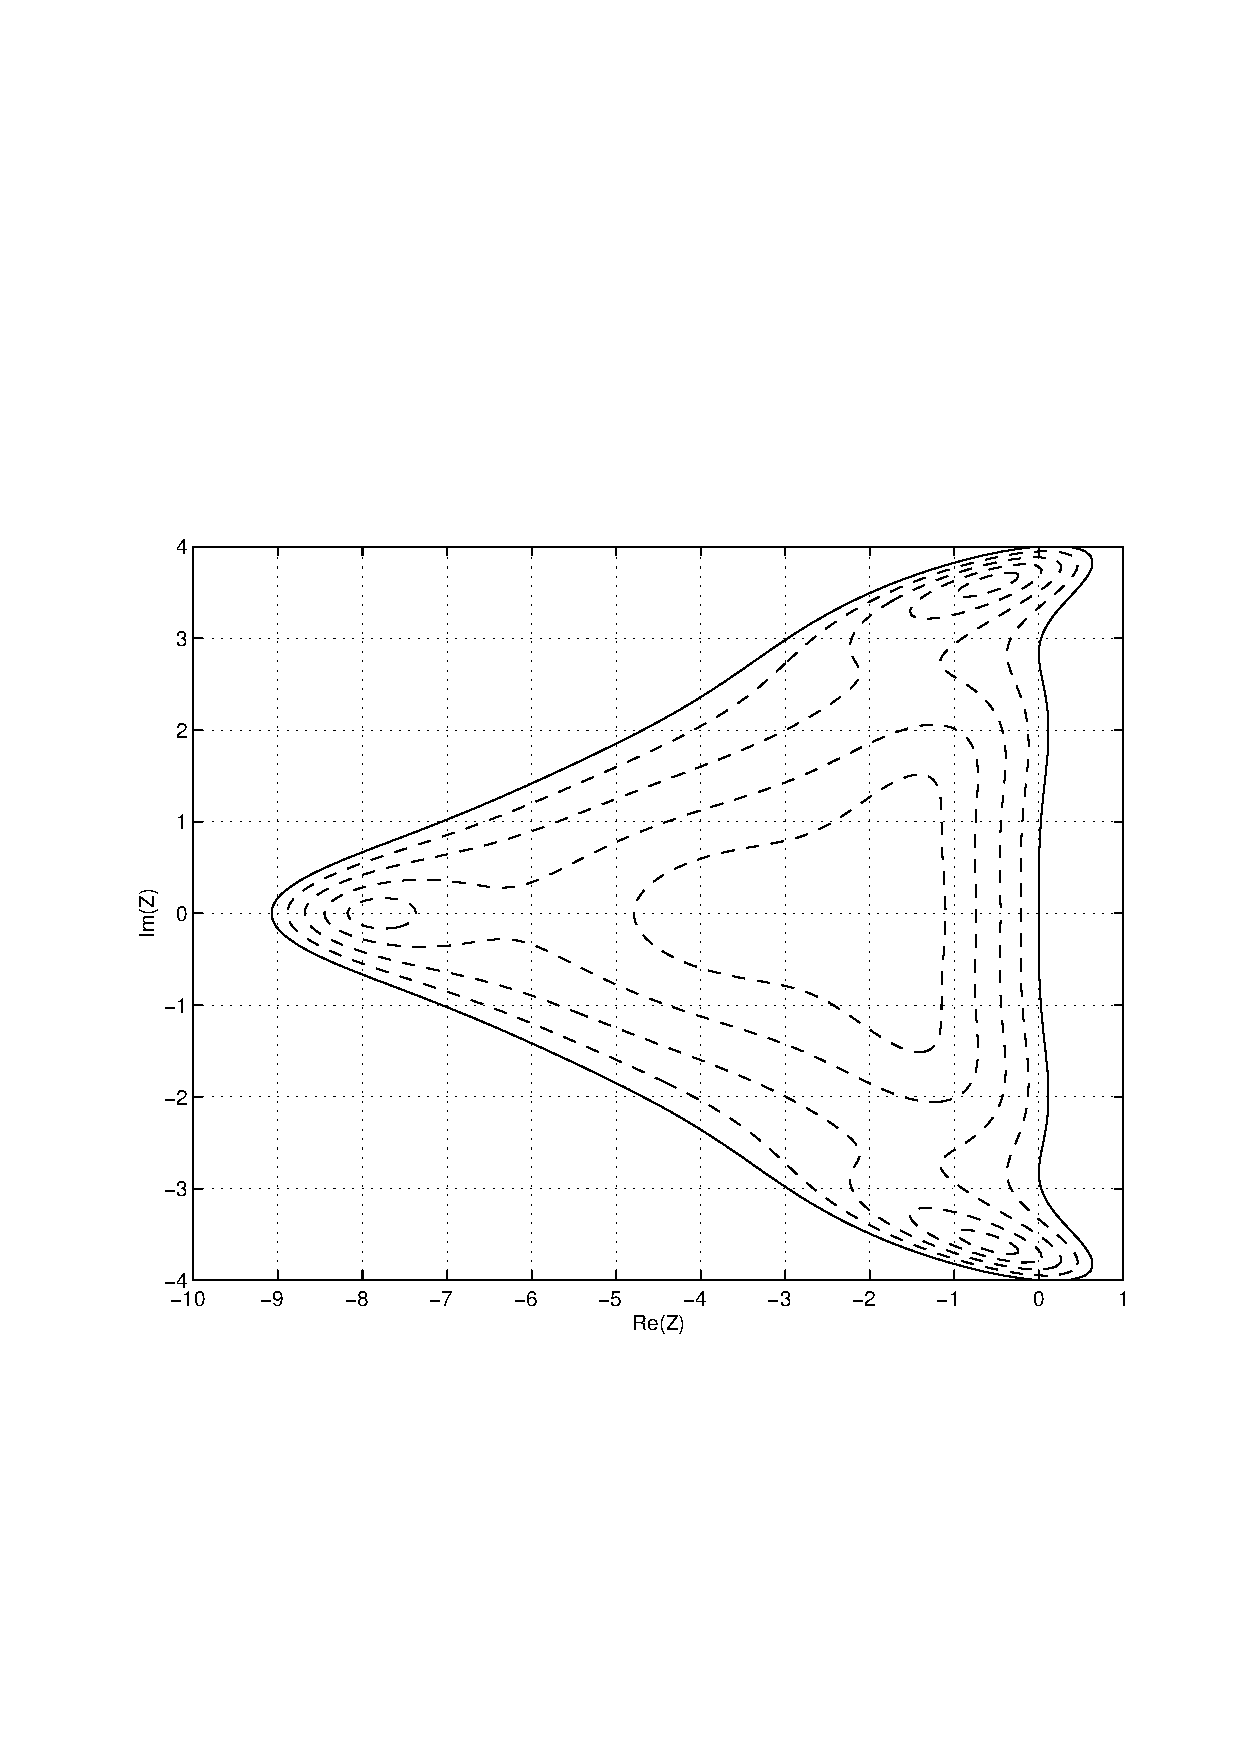
\includegraphics[width=100mm,clip=t]{APPEND/FIGURE/rk5.pdf}}
   \caption{Stability region and contours defined by
   $\left|\psi\left(Z\right)\right|=0.2, 0.4, ... 1$ for a 5-stage Runge-Kutta
    time stepping scheme.}
   \label{rk5.fig}
\end{figure}
%
 A first order spatial discretisation on the coarse levels is employed
 while retaining the second order accurate discretisation on the fine
 grid. This corresponds to the use of a defect-correction scheme on
 the coarser levels of the multigrid algorithm
 (Mavriplis \citeyearNP{Mavriplis:5}).
%
%
%
\subsection{Preconditioners}
%
 Following the approach of Pierce et al \citeyear{Giles:11},
 Mavriplis \citeyear{Mavriplis:6,Mavriplis:7},
 a point-implicit or a line-implicit Jacobi preconditioner has been
 used in order to give some degree of implicitness to the multistage
 scheme. The Jacobi preconditioner can be view as a characteristic
 time-step in contrast with a local time-step also called scalar
 preconditioner.
%
\paragraph{Point-implicit Jacobi Preconditioner}
%
 The point-implicit Jacobi preconditioner is based on the form of the discrete
 residual operator and is obtained by extracting the terms corresponding
 to the central node in the stencil.
 Referring to (\ref{semi_discrete_nl.eq}) and (\ref{semi_discrete_nl_2.eq})
 the point-Jacobi preconditioner $\left[{\bf P}\right]\se{-1}\sm{PJ}$ for a point $I$ is given by

%
\beq
  \left[{\bf P}\right]\sm{PJ}\se{-1} =
  - \frac{1}{\sigma}\frac{\partial {\bf R}\sm{I}}{\partial {\bf U}\sm{I}}
  = \frac{1}{\sigma}
   \sum\sm{s=1}\se{m\sm{I}}
   \left( \left|\vec{\eta}\sm{IJs}\right|\left|{\bf A}\sm{IJs}\right|
   + \tau\sm{IJs} \left.\frac{\partial {\cal G}{\scriptstyle l}\sm{IJs}}
                {\partial {\bf U}\sm{I}}\right|\sm{\mu}\right)
 \label{diagonal_jacobian.eq}
\eeq
%
 where $\sigma$ is the CFL number. In the derivation of (\ref{diagonal_jacobian.eq})
 the contribution of the source terms has been neglected.
 For the linearised Navier-Stokes
 equation the preconditioner assumes the same form and it is evaluated
 using the steady-state unknown, i.e.

%
\beq
  \left[\overline{\bf P}\right]\sm{PJ}\se{-1} =
   \frac{1}{\sigma}
   \sum\sm{s=1}\se{m\sm{I}}
   \left( \left|\vec{\eta}\sm{IJs}\right|\left|\overline{\bf A}\sm{IJs}\right|
   + \tau\sm{IJs} \left.\frac{\partial \overline{\cal G}{\scriptstyle l}\sm{IJs}}
                {\partial \overline{\bf U}\sm{I}}\right|\sm{\overline{\mu}}\right)
 \label{diagonal_jacobian_lin.eq}
\eeq
%
 $\left[{\bf P}\right]\sm{PJ}\se{-1}$ is a $5\times 5$ matrix which
 can be directly inverted using
 a standard algorithm.
 The preconditioner $\left[{\bf P}\right]\sm{PJ}\se{-1}$ has been obtained considering
 only the first order discretisation even when a second order scheme is used.
 This procedure is analogous to the practice of using a first order
 discretisation for the Jacobian in implicit methods (defect correction procedure).

 Note that for a scalar dissipation scheme, as the one by Jameson et al. \citeyear{Jame:1},
 the contribution of the artificial viscosity to $\left[{\bf P}\right]\sm{PJ}\se{-1}$ becomes
 diagonal and the scalar time-step estimate is recovered. Thus for
 a scalar dissipation scheme the smoother becomes a standard explicit multistage
 algorithm.

 In conjunction with preconditioner (\ref{diagonal_jacobian.eq}), no other
 techniques such as residual smoothing (Jameson \citeyearNP{Jame:1},
 Arnone \citeyearNP{Arnone:1}) are employed.
%
%
%
\paragraph{Line-implicit Jacobi Preconditioner}
%
 In computing high Reynolds number flows, with no-slip boundary condition
 at solid walls, the problem of grid anisotropy has been tackled by using
 a directional agglomeration multigrid strategy coupled with a line-implicit
 smoother.
 The combination of these two strategies into a single algorithm has been found to
 result in a more robust and efficient solution method than the use
 of either strategy alone (Mavriplis \citeyearNP{Mavriplis:6,Mavriplis:7}).

 Directional coarsening techniques were developed in order to overcome the problem related
 to the directional decoupling in highly stretched grids.
 Coarsening the grid in the stretching direction allows the smoother to efficiently damp
 the high error mode along the coarsening direction (Mulder \citeyearNP{Mulder:1},
 Pierce et al. \citeyearNP{Giles:11}). However standard directional coarsening techniques
 results in sequence of coarse grid levels for which the complexity between successive levels
 decreases by a factor of 2. The higher complexity of the directionally coarsened levels greatly
 increases memory overheads and make the use of multigrid W-cycles impractical
 (Mavriplis \citeyearNP{Mavriplis:6}).

 An alternative approach is obtained with a directional coarsening technique
 with a fine-to-coarse grid ratio of 4:1. In such case a more efficient smoother in the
 coarsening direction must be employed. This is obtained by using a
 lime-implicit preconditioner which achieves superior smoothing of error
 components along the direction of the implicit lines,
 as compared with the point-implicit method (Mavriplis \citeyearNP{Mavriplis:6,Mavriplis:7}).
 An example of line construction in the boundary layer region of a turbine blade
 is given in Fig. \ref{lines.fig}.

 The line-implicit Jacobi preconditioner is obtained by including the complete
 inviscid and Laplacian operators in the normal direction but only the component
 corresponding to the central node for the other directions.
 The resulting matrix represent a tridiagonal $5\times 5$ block system which
 has been solved using a Jacobi iterative procedure.
%
%
%
%
\section{Example}
\headd{Agglomeration Multigrid}{Example}
%
%
 The steady-state flow over a 2D turbine blade were used
 in order to assess the efficiency of the line-implicit preconditioner
 coupled with a full directional coarsening in the boundary layer.
 The directional line in this region are shown in Fig. \ref{lines.fig}
 while the control volumes of the fine mesh and three successively
 agglomerated grid are shown in Fig. \ref{agglo_mesh1.fig}
%
\begin{figure}[ht]
   \centerline{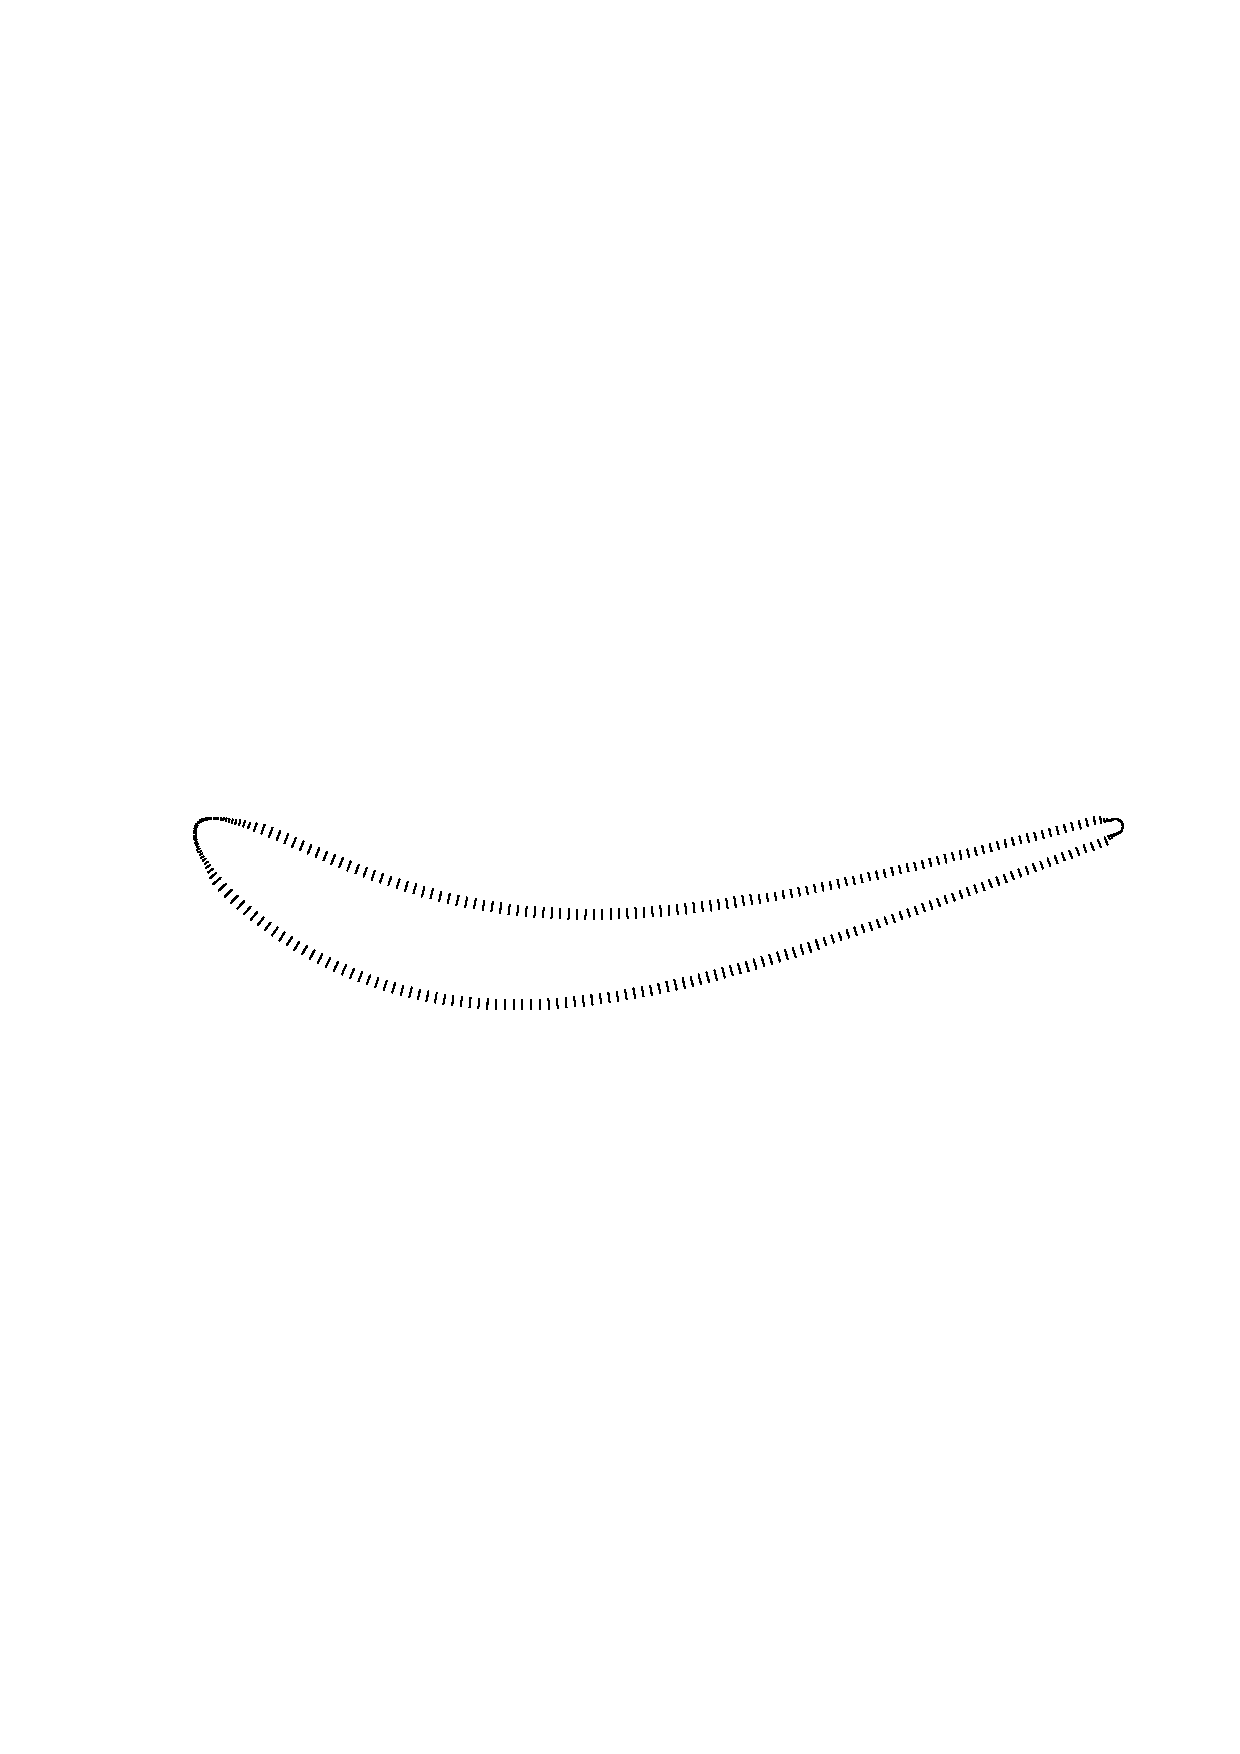
\includegraphics[width=120mm,clip=t]{APPEND/FIGURE/lines.pdf}}
  \caption{$11\se{th}$ Standard Configuration. Directional lines}
 \label{lines.fig}
\end{figure}
%
 The test case correspond to the $11\se{th}$ International Standard Configuration
 at transonic off-design conditions studied in Chapter \ref{linear.chap}.
%
\begin{figure}[ht]
 \begin{center}
  \begin{tabular}{cc}
    \subfigure[Fine grid]
       {\fbox{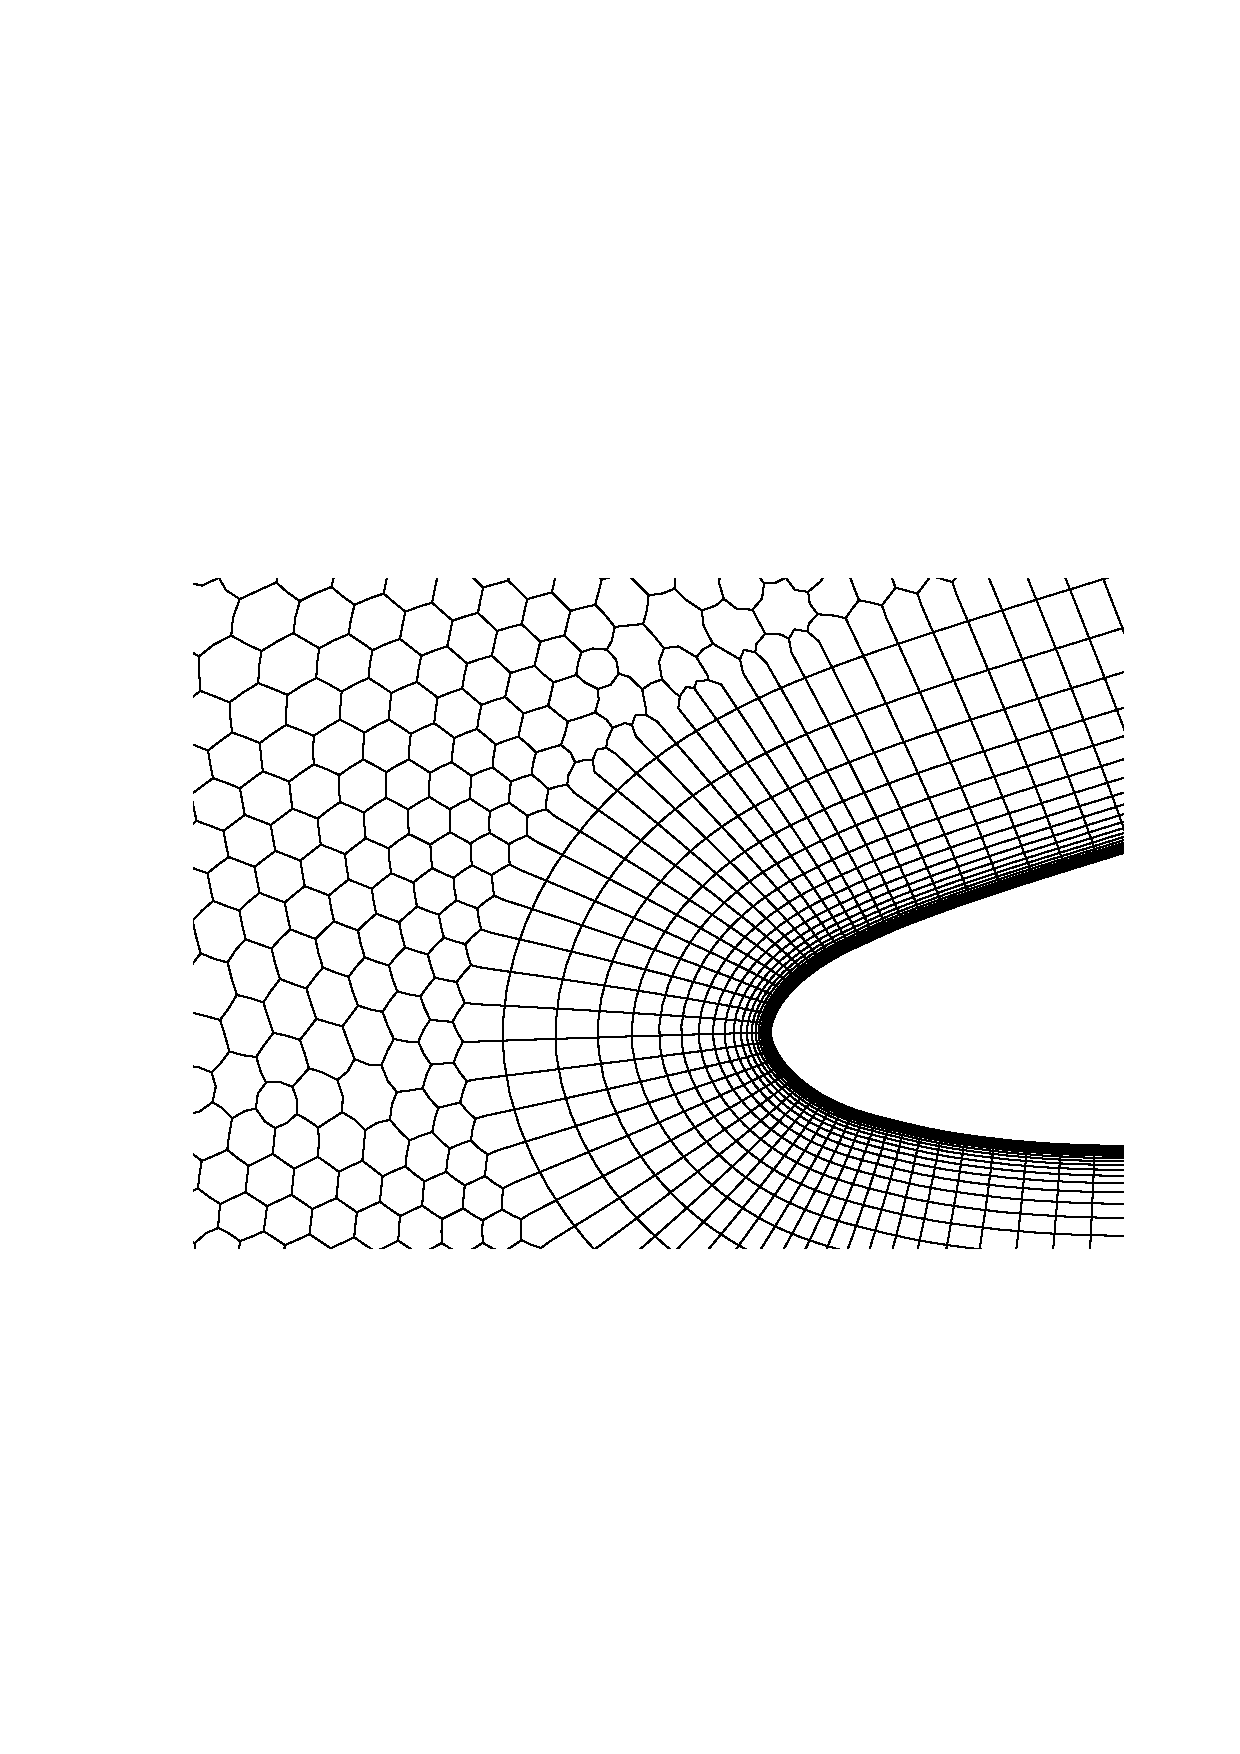
\includegraphics[width=60mm,clip=t]{APPEND/FIGURE/nose1.pdf}}}
        &
    \subfigure[grid 2]
       {\fbox{\includegraphics[width=60mm,clip=t]{APPEND/FIGURE/nose2.pdf}}}
       \\
    \subfigure[grid 3]
       {\fbox{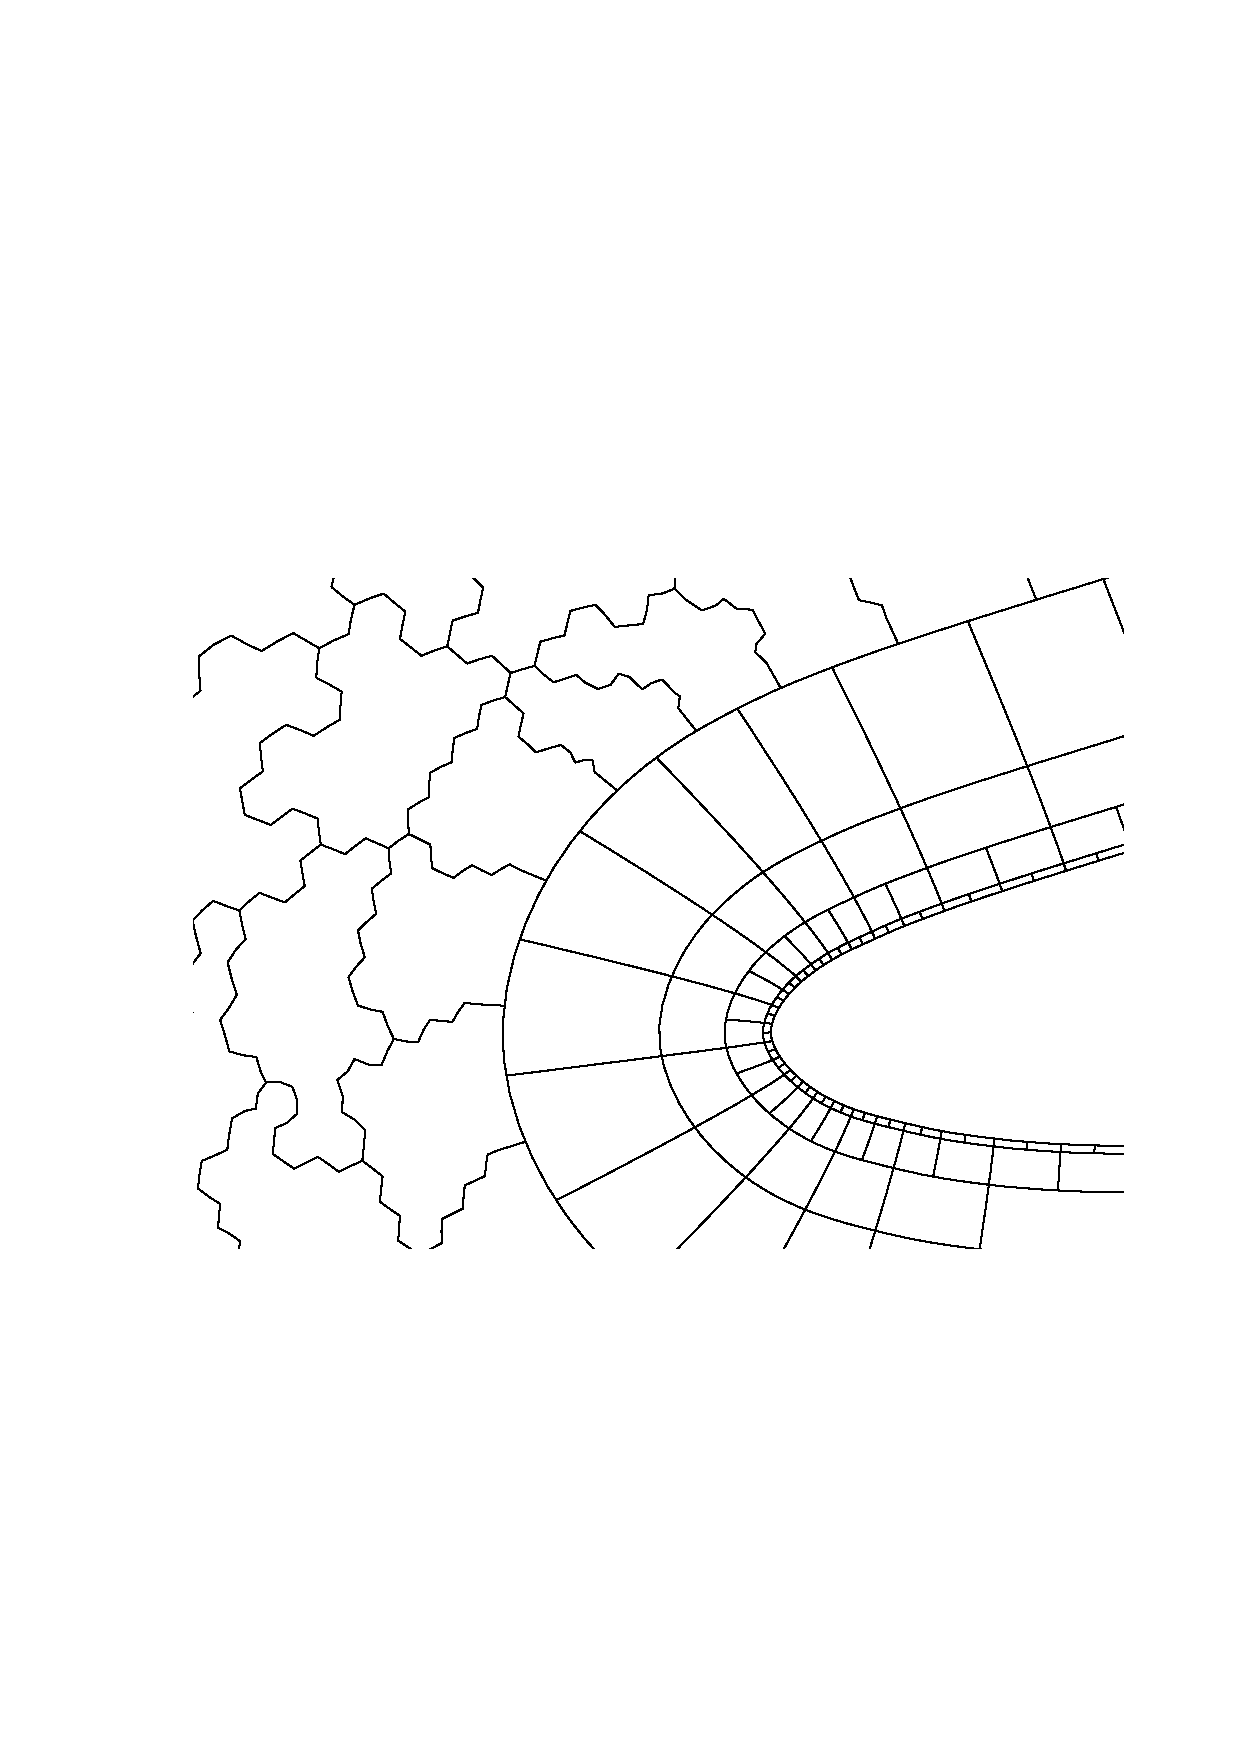
\includegraphics[width=60mm,clip=t]{APPEND/FIGURE/nose3.pdf}}}
        &
    \subfigure[grid 4]
       {\fbox{\includegraphics[width=60mm,clip=t]{APPEND/FIGURE/nose4.pdf}}}
  \end{tabular}
 \end{center}
 \caption{$11\se{th}$ Standard Configuration (turbulent flow calculation
          up to the wall). Agglomerated control volumes}
 \label{agglo_mesh1.fig}
\end{figure}
%
%
 Fig. \ref{conver_app1.fig} show the convergence history of the density residual
 using two and four grids in a W-type cycle. The convergence history of
 the implicit (single grid) method of Sayma et al. \citeyear{Luca:10}
 is also plotted.
%
%
%
\begin{figure}[ht]
   \centerline{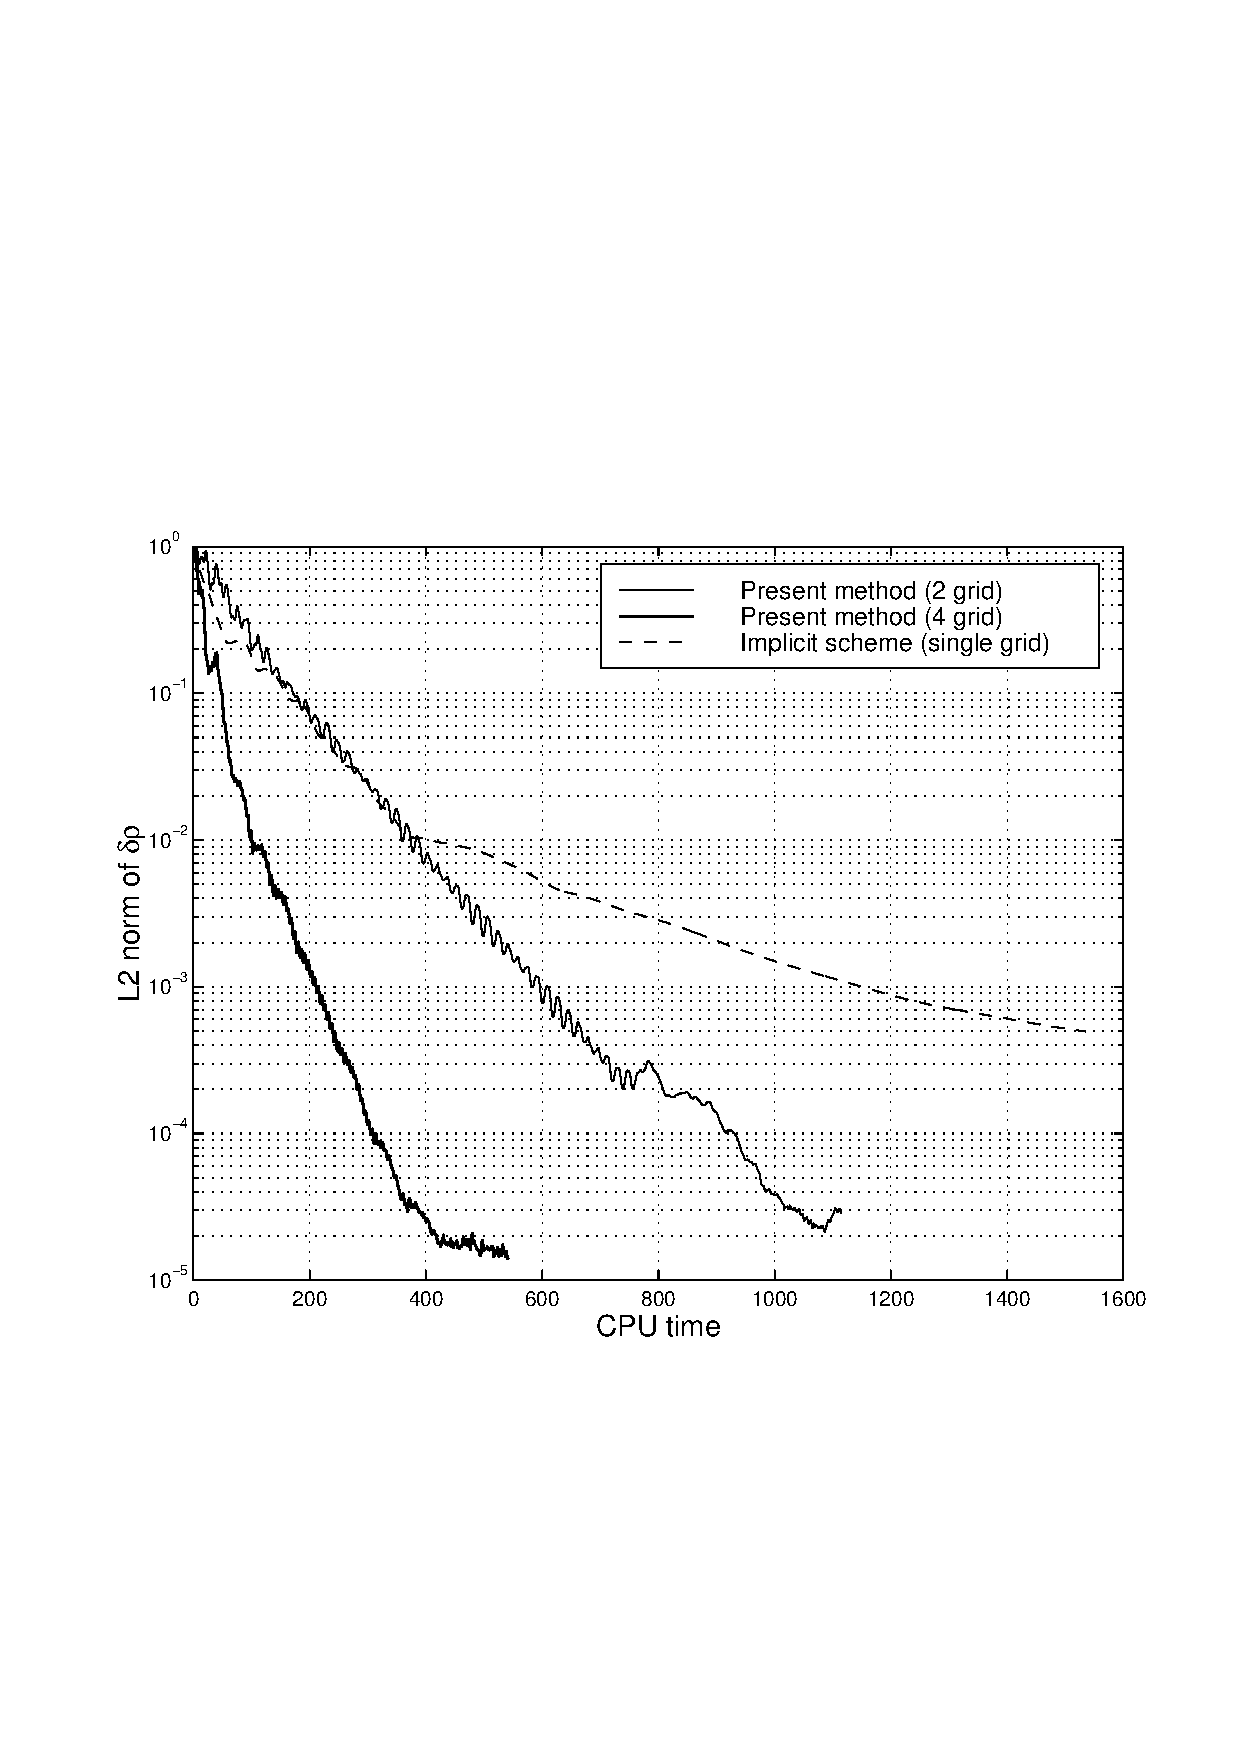
\includegraphics[width=120mm,clip=t]{APPEND/FIGURE/conv1.pdf}}
  \caption{$11\se{th}$ Standard Configuration (turbulent flow calculation
          up to the wall): convergence histories}
 \label{conver_app1.fig}
\end{figure}
%
%
%
\section{Concluding Remarks}
%
 (i) Efficient steady-state and linearised unsteady calculations can
 be performed using the multigrid relaxation scheme presented in the Appendix.
 The line-Jacobi preconditioner is used for turbulent viscous flow solved up to
 the wall while the point-Jacobi version is used for the other flow
 representations.
%
 (ii) The preconditioned agglomeration multigrid needs to be improved in order to
 enhance both performance and robustness, especially in 3D.
 A more accurate prolongation operator
 need to be developed. This task is non-trivial because of the absence
 of an underlying grid. The preconditioner may cause some instabilities
 at stagnation points, where large variations of the flow angle appear
 at significant velocity values. This loss of robustness can be attributed to
 a flow-angle sensitivity thus improvement in this direction should be made.
